% !TeX root = ../main.tex
% Preamble
\documentclass[../main.tex]{subfiles}
\graphicspath{{\subfix{../images/}}}


\begin{document}

\section{MPC protocol}
We now describe our implementation of an actively secure MPC protocol.

For this protocol we did not implement the cyclotomic polynomial optimisation described earlier, so $s = 1$, meaning that we are working in $\mathbb{F}_{p^k}$.
This also means that we cannot do entry-wise multiplications like done in \cite{damgaard2012multiparty}.
Therefore, to encode an element $a \in \mathbb{F}_{p^k}$ to an element in $R_p$, we simply return \lstinline{Polynomial::new(vec![a])}, which is the \lstinline{Polynomial} corresponding to $f(x) = a$. To decode a polynomial $f(x) = a \in R_p$, we simply return the \lstinline{Integer} $a$.

\subsection{Dealer and Player}

There are two types of actors in this system, the \textit{dealer} and the \textit{player}.

The \textit{dealer} acts as a trusted party for establishing connections between all parties and, once all parties have connected, provides the parties with key material (i.e. a public key and shares to the corresponding secret key), enabling distributed decryption.
For practical purposes, all players only need to know the address of the dealer, who will then forward the receiving addresses of all players to each other, enabling point-to-point communication.

All other parties in the protocol are \textit{players}.
A player contributes some private input to the function being computed, in the end receiving only the result and no other information.

To prepare for computing the agreed function, all players connect to the dealer, sending a "Start" message with their address for receiving TCP connections, and getting back a list of players who have already connected to the dealer (along with themselves).
Each player's position in this list indicates their "player number", which is relevant for some parts of the protocol.
When all players have connected, and all of the key material has been distributed, the dealer shuts down, as it is no longer needed.
This is also described in figure \ref{fig:dealer-player}.

\begin{figure}
    \centering
    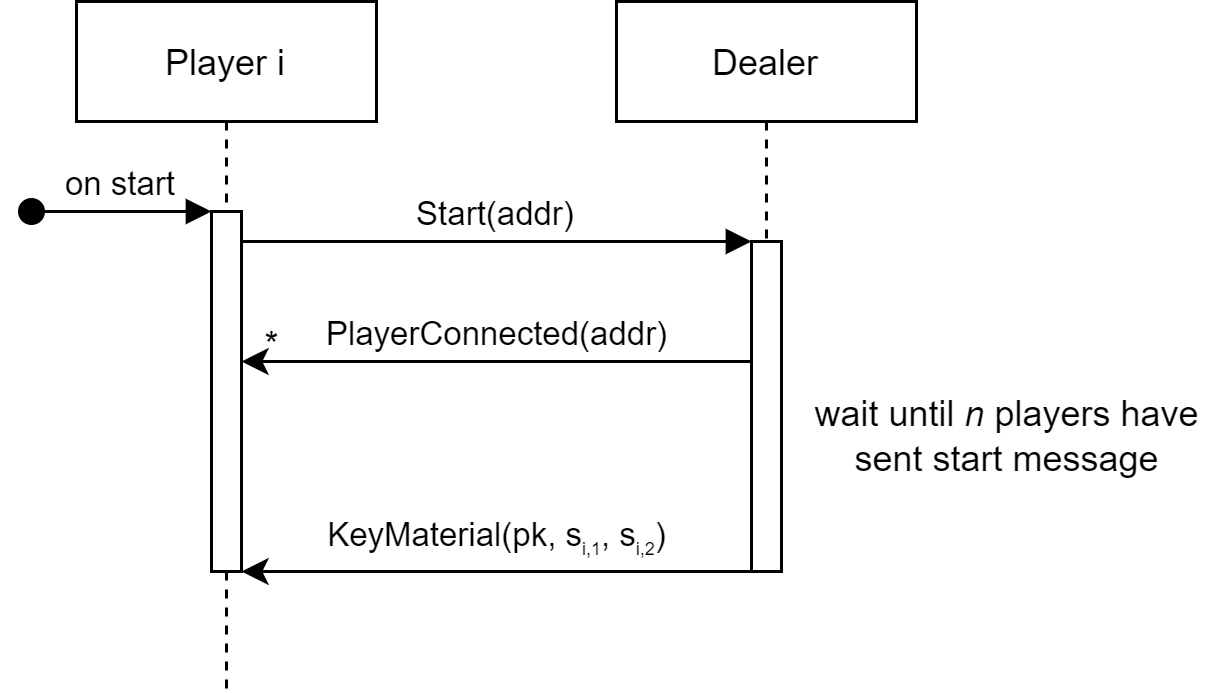
\includegraphics[width=0.8\textwidth]{Player-Dealer.png}
    \caption{A sequence diagram describing the protocol for player initialization using the trusted dealer.}
    \label{fig:dealer-player}
\end{figure}

\subsubsection{Facilitator}

The \lstinline{Facilitator} is a small, but central component that enables communication between the parties while running the protocol.
While it is not a theoretically important part of the system, it ended up being used in almost all other components, and will therefore be summarized here.

After the dealer has shut down, each player uses a \lstinline{Facilitator} to communicate with the other players, providing functions for broadcasting or sending point-to-point messages (\lstinline{broadcast} and \lstinline{send}), as well as for receiving messages from a designated player or from all players at once (\lstinline{receive} and \lstinline{receive_from_all}).

To ensure that all messages are received in the desired order, sending a message is handled entirely synchronously for the player (i.e. the \lstinline{send} function is handled in the main thread, and therefore will not return until the message has been accepted by the other party).

Oppositely, receiving messages is handled by a dedicated thread that holds a \lstinline{TCPListener} (the one for which the address was published).
Once a messages is received, it is added to a channel corresponding to the player that sent the message, ready to be read whenever the receiving player is ready.
If no message is ready, the \lstinline{receive} function blocks until a message is received.

The system currently does not have any mechanism for verifying the origin of messages, as a new connection is opened on a new port each time a player wants to send a message to another player.
Therefore, each player sends along their own identity when sending a message, which would obviously be insecure in a production-ready system.
This issue could be resolved in many ways, for example using public-key cryptography and authenticated channels.

\subsubsection{PlayerState}

The \lstinline{PlayerState} struct is also frequently used in our implementation. Similarly to the \lstinline{Parameters} struct, it is a container for most of the values that need to be known by the player for most of the MPC protocol.

It includes the key material received from the dealer $(pk, s_{i,1}, s_{i,2})$, our share of the global MAC key $\alpha_i$, the encrypted global key $e_\alpha$, a list of pairs $(a, \gamma(a)_i)$ (where $a$ is a value that has been opened, and $\gamma(a)_i$ is our share of $\alpha a$), and a \lstinline{Facilitator} instance.

\subsection{Distributed decryption}
The \lstinline{ddec} function implements the distributed decryption part of the $\mathcal{F}_{KeyGenDec}$ functionality described earlier. The function takes a \lstinline{Parameters} struct \lstinline{params}, a \lstinline{PlayerState} \lstinline{state}, and a mutable \lstinline{Ciphertext} \lstinline{c} as arguments.

First we check if \lstinline{c} contains $3$ elements, and if this is not the case then we pad the ciphertext with a $0$, since we need there to be three entries for the following computations.

If it is $P_1$ calling the method, then we use our quotient ring implementation to compute
\begin{center}
    \lstinline{v_i = c[0] + state.sk_i1 * c[1] + state.sk_i2 * c[2]}
\end{center}
otherwise we compute
\begin{center}
    \lstinline{v_i = state.sk_i1 * c[1] + state.sk_i2 * c[2]}
\end{center}

Now we use \lstinline{sample_from_uniform} to sample a polynomial with $\ell_\infty$ norm bounded by $2^{sec} \cdot B/(n \cdot p)$, meaning that the coefficients are in the interval $[0, 2^{sec} \cdot B/(n \cdot p)]$, where $B$ is a bound on the $\ell_\infty$ norm of $t$.
The reason why we let the coefficients depend on $B$, is that we do not want to add too much noise, since this would result in decryption returning the incorrect result.

We then add $p$ times the polynomial that we just sampled to $v_i$, so that we get $t_i$. Adding this randomness corresponds to drowning the noise of the ciphertext as described in the section on circuit security.

Following this we broadcast $t_i$, and then receive the other players shares, which allows us to compute $t' = t_1 + ... + t_n \mod p$.

We then normalize the coefficients of $t'$ to get \lstinline{msg_minus_q} like done in \lstinline{decrypt}, so that they are in the interval $[-q/2, q/2)$.

Finally, we compute \lstinline{msg_mod_q.modulo(&params.p)}, then call decode on the result to get an Integer which we return.

\subsection{ZKPoPK (mpc/zk.rs)}

In zk.rs the zero knowledge proof of plaintext is implemented for each party to run.
The zero-knowledge proof has been implemented as in figure 10 of ``multiparty computation from somewhat homomorphic encryption''~\cite{damgaard2012multiparty}.
The file is divided into 2 different functions.
To generate a zero knowledge proof, we must call the function make\_zkopk() which takes 6 arguments
\begin{itemize}
    \item \textbf{params} The parameters of the PLWE instantiation.
    \item \textbf{x}: The plaintext for which we intend to generate the proof.
    \item \textbf{r}: The randomness to be used.
    \item \textbf{c}: The ciphertexts generated in the preprocessing protocol.
    \item \textbf{diag}: A boolean to indicate whether the diagonal element should be checked.
    \item \textbf{Pk}: The public key to be used.
\end{itemize}
make\_zkopk() will generate 3 values $(a, z, T)$, which will be used in the verification of the proof.
To verify the proof we call the function verify\_zkopk, which takes as input 6 arguments as well
\begin{itemize}
    \item \textbf{a}: value generated by the make\_zkopk function.
    \item \textbf{z}: value generated by the make\_zkopk function.
    \item \textbf{t}: value generated by the make\_zkopk function.
    \item \textbf{c}: The ciphertexts generated in the preprocessing protocol.
    \item \textbf{params} The parameters of the PLWE instantiation.
    \item \textbf{Pk}: The public key to be used.
\end{itemize}
verify\_zkopk will return a boolean indicating whether or not the proof was valid.
% TODO: vores matrix beregninger har dimensioner omvendt, men det er fikset ved at gå anderledes igennem matrixen.

\subsection{Preprocessing phase (mpc/prep.rs)}
The file \lstinline{prep.rs} contains all of the functions that are called in the preprocessing phase to generate values for the online phase.

The functions \lstinline{reshare} and \lstinline{p_angle} correspond to the Reshare and PAngle protocols explained previously, while \lstinline{initialize}, \lstinline{pair}, and \lstinline{triple} correspond to three steps of the Prep protocol.

The file also contains a type definition \lstinline{AngleShare}, which for some value $\langle v \rangle$ is a pair of the form $(v_i, \gamma(v)_i)$ for some player $i$. Additionally, the file also contains a definition \lstinline{MulTriple}, which contains three \lstinline{AngleShare} values, and represent a players shares of the $\langle \cdot \rangle$ values in a multiplicative triple. %TODO: Faktisk i mod.rs åbenbart

\subsubsection{reshare}
The first function, \lstinline{reshare}, takes as input a \lstinline{Parameters} struct \lstinline{params}, a Ciphertext \lstinline{e_m}, a  \lstinline{PlayerState} \lstinline{state}, and an \lstinline{Enc} enum \lstinline{enc}, which can take on values \lstinline{NewCiphertext} or \lstinline{NoNewCiphertext}.

The first thing done in this function is to sample a value \lstinline{f_i} uniformly from $Z_p$ using \lstinline{sample_single} from \lstinline{prob.rs}. Then, \lstinline{f_i} is encrypted to get \lstinline{e_f_i}.
%Mangler ZK
The facilitator is then used to broadcast \lstinline{e_f_i}, and subsequently receive the encrypted shares from the other parties, which are then homomorphically added to get \lstinline{e_f}. Then, we compute \lstinline{e_m_plus_f = add(params, e_m, &e_f)}.

The \lstinline{ddec} function from mod.rs is then called with \lstinline{e_m_plus_f} as input to get the plaintext \lstinline{m_plus_f}.

Then we set \lstinline{m_i} to be $e_{m + f} - f_i \text{ mod } p$ if the player calling the function is the player with index $0$, and $- f_i \text{ mod } p$ otherwise. If \lstinline{enc = NewCiphertext}, we now encrypt \lstinline{m_plus_f} using \lstinline{encrypt_det} where we use a triple of 1-polynomials instead of the randomness to make encryption deterministic. Now, we use \lstinline{add} from encrypt.rs to homomorphically subtract the encrypted shares $e_{f_i}$ from the encryption of \lstinline{m_plus_f} to get \lstinline{e_m_prime}. Afterwards, we return \lstinline{(Some(e_m_prime), m_i)}

If \lstinline{enc = NoNewCiphertext}, we instead just return \lstinline{(None, m_i)}.

\subsubsection{p\_angle}
The \lstinline{p_angle} function takes a \lstinline{Parameters} struct \lstinline{params}, an \lstinline{Integer} \lstinline{v_i}, a \lstinline{Ciphertext} \lstinline{e_v}, and a \lstinline{PlayerState} \lstinline{state} as input.

The first thing done in \lstinline{p_angle} is to homomorphically multiply \lstinline{e_v} and \lstinline{state.e_alpha} to get \lstinline{e_v_mul_alpha}. Then, \lstinline{reshare} is called to get \lstinline{gamma_i}, which is a share of an \lstinline{Integer}, namely the plaintext in \lstinline{e_v_mul_alpha}. Lastly, the function returns \lstinline{(v_i, gamma_i)}, which is an \lstinline{AngleShare} value corresponding to a share of $\langle v \rangle$.

As can be seen from the implementation we omit the public $\delta$ value as done in \cite{damgaard2013practical}, such that the MAC's now instead satisfy $\alpha v = \sum_i \gamma(v)_i$.
 
\subsubsection{initialize}
The initialize function takes a \lstinline{Parameters} struct \lstinline{params}, and a mutable \lstinline{PlayerState} \lstinline{state} as input.

First, we sample a uniformly random \lstinline{Integer} from $Z_p$ using the \lstinline{sample_single} function with \lstinline{params.p} as input, and set the \lstinline{alpha_i} variable of the player state to this value. This represents the given players share of the global key. We then encrypt \lstinline{state.alpha_i} to get an encrypted share \lstinline{e_alpha_i}. Now, \lstinline{e_alpha_i} is broadcast using \lstinline{state.facilitor}, and each player then uses their facilitator to receive $e_{\alpha_i}$ from the other players. The $e_{\alpha_i}$'s are then homomorphically added to get $e_\alpha$, and the result is then assigned to the \lstinline{e_alpha} variable of \lstinline{state}. %Well ikke helt, men add_encrypted_shares, skal vi nævne det?
Finally, we run \lstinline{zpopk} from \lstinline{zk.rs} in a loop $sec$ times.

Notice how we do not compute the personal keys $\beta_i$ as done in \cite{damgaard2012multiparty}. As mentioned earlier these are not needed when we use the trick described in section \ref{section: Reuse}.
\subsubsection{pair}
The \lstinline{pair} function takes a Parameters struct params, and a PlayerState state as input.

The function first samples a uniformly random \lstinline{Integer} \lstinline{r_i} from $Z_p$. Now, \lstinline{r_i} is encrypted to get \lstinline{e_r_i}, which is the broadcast using the facilitator. All players then again use the facilitator to receive the encrypted shares from the other parties, which are then homomorphically added to compute \lstinline{e_r}. Then, we call \lstinline{zkpopk} with \lstinline{e_r_i} as input.

Following this we compute the given players share of $\langle r \rangle$ with a call to \lstinline{p_angle} with \lstinline{r_i} and \lstinline{e_r} as arguments, which returns \lstinline{r_angle}.

Again, we use the trick explained in section \ref{section: Reuse}, so we don't need the values in the bracket representation, and therefore we just return \lstinline{(r_i, r_angle)}, which corresponds to shares of the pair $(r, \langle r \rangle)$.

\subsubsection{triple}
The triple function takes a \lstinline{Parameters} struct \lstinline{params}, along with a \lstinline{PlayerState} \lstinline{state} as arguments.

First, we sample \lstinline{a_i}, \lstinline{b_i} uniformly at random from $Z_p$, which are both then encrypted, and the encrypted shares are then broadcast.

Then, when the player receives the encrypted shares of $a$ and $b$ from the other players, then these are homomorphically added to get \lstinline{e_a} and \lstinline{e_b}.

Following this, we generate shares \lstinline{a_angle} and \lstinline{b_angle} with calls to \lstinline{p_angle} using \lstinline{a_i}, \lstinline{e_a} and \lstinline{b_i}, \lstinline{e_b} as input respectively.

Now, the player calling the function has shares of $\langle a \rangle$ and $\langle b \rangle$, and we need to compute a share of $\langle c \rangle$.

To do this we compute \lstinline{e_c} by homomorphically multiplying \lstinline{e_a} and \lstinline{e_b}, and then we call \lstinline{reshare} with \lstinline{e_c} and \lstinline{NewCiphertext} as input to get a new ciphertext \lstinline{e_c_prime} and \lstinline{c_i}, which is a share of c. 

This allows us to call \lstinline{p_angle} using \lstinline{c_i} and \lstinline{e_c_prime} to get \lstinline{c_angle}.

Finally, we return a \lstinline{MulTriple} containing \lstinline{a_angle}, \lstinline{b_angle}, and \lstinline{c_angle}.

\subsection{Commitments (mpc/commit.rs)}
For the online phase we also need a commitment functionality as described in \cite{damgaard2013practical}.
Our implementation of this functionality can be found in commit.rs. This file contains the methods \lstinline{commit} and \lstinline{open}, which are explained in greater detail below.

\subsubsection{commit}
The commit function simply takes two \lstinline{Vec<u8>} values called \lstinline{v} and \lstinline{r}, along with a \lstinline{PlayerState} \lstinline{state} as input. Then \lstinline{v} is the value that we wish to commit to, while \lstinline{r} is the randomness that we use when committing.

In this method we utilize the implementation of sha256 found in the \lstinline{sha2} package to hash the concatenation of \lstinline{v} and \lstinline{r}, which yields the commitment \lstinline{c}.

\lstinline{c} is then broadcast to all players using the facilitator.

\subsubsection{open}
This function takes a commitment \lstinline{c} and a value \lstinline{o} as input, and these are both \lstinline{Vec<u8>}. The \lstinline{o} value is then supposed to satisfy that $o = v || r$.

When calling this function it hashes \lstinline{o} using sha256, and then checks whether \lstinline{h(o) = c}. If this is indeed the case, then we return \lstinline{Ok(o)}, and otherwise we return an error.

\subsection{Online phase (mpc/online.rs)}
The code related to the online phase can be found in \lstinline{mpc/online.rs}. The implementation of this phase is based on the online protocol in \cite{damgaard2013practical}, but in that protocol the triple check is done in preprocessing, while we do it in the online phase as in \cite{damgaard2012multiparty}.

The two functions \lstinline{give_input} and \lstinline{receive_input} together correspond to the Input step of the protocol.
The \lstinline{add}, \lstinline{multiply}, and \lstinline{output} functions correspond to the steps of the same names.
The function \lstinline{maccheck} corresponds to the MACCheck protocol, and \lstinline{triple_check} is used as a subroutine in \lstinline{multiply} to check for validity of a multiplicative triple.

\subsubsection{give\_input}
This function takes a \lstinline{Parameters} struct \lstinline{params}, an \lstinline{Integer} \lstinline{x_i}, a \lstinline{(Integer, AngleShare)} pair called \lstinline{r_pair}, and a \lstinline{PlayerState} \lstinline{state}.

First, the function broadcasts a message \lstinline{BeginInput} to indicate that the player calling the function wants to give some input.

Then, the player receives all shares of $r$ from the other players using the facilitator, and opens $r$ by computing $r = r_1 + ... + r_n \mod p$.

The value \lstinline{eps = x_i - r} is then computed, and subsequently broadcast to all players.

The \lstinline{AngleShare} corresponding to $\langle r \rangle + \epsilon$ is then computed and returned.
\subsubsection{receive\_input}
The \lstinline{receive_input} function takes a \lstinline{Parameters} struct \lstinline{params}, an \lstinline{Integer} \lstinline{x_i}, a \lstinline{(Integer, AngleShare)} pair called \lstinline{r_pair}, and a \lstinline{PlayerState} \lstinline{state}.

The first thing that the function does is to receive a message using the facilitator, and if this is not \lstinline{BeginInput}, then we panic.

Following this we take $r_i$ from \lstinline{r_pair}, and send it to the player \lstinline{p_i}, which is the player that is providing input, and thus also the player that sent the initial \lstinline{BeginInput} message.

Now, we receive $\epsilon$ from \lstinline{p_i}, and then use this to compute and return the \lstinline{AngleShare} corresponding to $\langle x_i \rangle = \langle r \rangle + \epsilon$ for the given player.

\subsubsection{add}
Add simply takes two \lstinline{AngleShare} values \lstinline{x} and \lstinline{y} as input.

These are then used to compute \lstinline{(x.0 + y.0, x.1 + y.1)}, and the resulting \lstinline{AngleShare} is then returned.
\subsubsection{partial\_opening}
To partially open some value $v$ where player $i$ holds share $v_i$, each player calls \lstinline{partial_opening} with a \lstinline{Parameters} struct \lstinline{params}, an \lstinline{Integer} \lstinline{to_share}, and a \lstinline{PlayerState}  \lstinline{state} as arguments. When partially opening we send all shares to some designated player, and in this case we simply let all players send their share to player $P_1$, who has index $0$.

To do this we first send the calling players share of $v$, \lstinline{to_share}, to $P_1$ using the facilitator. Player $P_1$ then computes $v = v_1 + ... + v_n \mod p$, which is subsequently broadcast to all players using the facilitator.

Finally, the function returns the value $v$ received from $P_1$.

\subsubsection{triple\_check}
The \lstinline{triple_check} function takes a \lstinline{Parameters} struct \lstinline{params}, two \lstinline{MulTriple} values \lstinline{abc_triple} and \lstinline{fgh_triple}, an \lstinline{Integer} \lstinline{t_share}, and a mutable \lstinline{PlayerState} \lstinline{state} as arguments.

The first thing done is to use the facilitator to broadcast the players share of $t$, \lstinline{t_share}. The player then uses the facilitator to receive shares of $t$ from the other players, and then compute $t = t_1 + ... + t_n \mod p$.

Now, we compute $t \cdot \langle a \rangle - \langle f \rangle$ and save the resulting \lstinline{AngleShare} in variable \lstinline{rho_share}. Following this we call \lstinline{partial_opening} with \lstinline{rho_share.0} as input to get $\rho$. Lastly, we push \lstinline{(rho, rho_share.1)} to \lstinline{state.opened}, to ensure that we check the MAC of $\rho$ in \lstinline{maccheck}.

Now, we use the same approach as for $\rho$ to compute $\langle b \rangle - \langle g \rangle$ and store the resulting \lstinline{AngleShare} in variable \lstinline{sigma_share}. Then we call \lstinline{partial_opening} with \lstinline{sigma_share.0} as input to get $\sigma$. Then we push \lstinline{(sigma, sigma_share.1)} to \lstinline{state.opened}.

We then compute $t \cdot \langle c \rangle - \langle h \rangle - \sigma \cdot \langle f \rangle - \rho \cdot \langle g \rangle - \sigma \cdot \rho$, call \lstinline{partial_opening} with the resulting \lstinline{AngleShare} as input to get the variable \lstinline{zero}.

The last thing done is to check whether \lstinline{zero} is $0$. If this is the case, then we return \lstinline{Ok}, otherwise we return \lstinline{Err}.

\subsubsection{multiply}
The \lstinline{multiply} function takes a \lstinline{Parameters} struct \lstinline{params}, two \lstinline{AngleShare} values \lstinline{x} and \lstinline{y}, two \lstinline{MulTriple} values \lstinline{abc_triple} and \lstinline{fgh_triple}, an \lstinline{Integer} \lstinline{t_share}, and a \lstinline{PlayerState} \lstinline{state} as arguments.

First, we call \lstinline{triple_check} with \lstinline{params}, \lstinline{abc_triple}, \lstinline{fgh_triple}, \lstinline{t_share}, and \lstinline{state} as input. If the call to \lstinline{triple_check} returns \lstinline{Err}, then we panic and abort the protocol, otherwise we proceed.

Following this we compute the AngleShare corresponding to $\langle x \rangle - \langle a \rangle$, so that we get \lstinline{eps_share}. We then call \lstinline{partial_opening} with \lstinline{eps_share.0} as input to get \lstinline{eps}. Then we push \lstinline{(eps, eps_share.1)} to \lstinline{state.opened}.

Now we compute the AngleShare corresponding to $\langle y \rangle - \langle b \rangle$, so we get \lstinline{delta_share}, then call \lstinline{partial_opening} with \lstinline{delta_share.0} as input to get \lstinline{delta}. And now we push \lstinline{(delta, delta_share.1)} to \lstinline{state.opened}.

Finally, we compute the \lstinline{AngleShare} corresponding to $\langle z \rangle = \langle c \rangle + \epsilon \langle b \rangle \delta \langle a \rangle + \epsilon \delta$ and return it.
\subsubsection{maccheck}
The \lstinline{maccheck} function takes a \lstinline{Parameters} struct \lstinline{params}, a \lstinline{Vec<(Integer, Integer)>} of $t$ $(a_j, \gamma(a_j)_i)$ pairs named \lstinline{to_check}, and a \lstinline{PlayerState} \lstinline{state} as arguments.

First, we use the \lstinline{rand} package to sample random $32$-byte values  \lstinline{s_i} and \lstinline{r}.

Then we use the \lstinline{commit} function from \lstinline{commit.rs}, to commit to \lstinline{s_i} using \lstinline{r} as randomness.

Following this we use the facilitator to receive the commitments from all $n$ parties. Then once all of the commitments have been received the parties broadcast the value $o = s_i || r$, such that all parties then open the commitments that they have received and get the seed $s_i$ for all players $i$.

Now, we XOR the received seeds to get $s = s_1 \oplus ... \oplus s_n$. This is followed by using the \lstinline{rand} package and the seed $s$ to sample a vector \lstinline{r} with $t$ entries and with values in the range $[0, p)$.

Then the function uses the values $a_1, ..., a_t$ stored in \lstinline{state.opened} to compute $a = \sum^t_{j = 1} r_j a_j$.

After generating $a$ we use it to compute $\gamma_i = \sum^t_{j = 1} r_j \gamma(a_j)_i$ and $\sigma_i = \gamma_i - \alpha_i a$. Then we convert $\sigma_i$ to bytes and store the result in \lstinline{sigma_i_bytes}.

Afterwards we need to commit to \lstinline{sigma_i_bytes}, and to do this we sample $32$ bytes of randomness \lstinline{r} as done earlier. This is followed by committing to \lstinline{sigma_i_bytes} using \lstinline{r} as randomness.

Now we use the facilitator to receive commitments from all $n$ players, and once these have been received we broadcast $o = sigma\_i\_bytes || r$.

Then we use the $o$ values received to open the $\sigma$ commitments received earlier, such that we get bytes corresponding to $\sigma_i$ from all players $i$. Then, we convert the bytes into values of the \lstinline{Integer} type.

Finally, we add the $n$ $\sigma_i$ values received and check that indeed the sum is equal to \lstinline{Integer::ZERO}. If this is the case, then we return true, otherwise we return false.

\subsubsection{output}
The \lstinline{output} function is called by a player when that player is ready to output some value $\langle y \rangle$. The function takes a \lstinline{Parameters} struct \lstinline{params}, \lstinline{AngleShare} \lstinline{y_angle}, and a \lstinline{PlayerState} \lstinline{state} as arguments.

To output a value we first call the \lstinline{maccheck} function on \lstinline{state.opened}, to check that the MAC values are correct for all of the values $v$ in the $\langle r \rangle$ representation that have been opened. If this returns false, then the check was unsuccessful and we \lstinline{panic} to abort the protocol.

Then we broadcast \lstinline{y_angle.0}, which is the players share $y_i$ of the output value $y$. This is followed by receiving shares from all players, and then computing $y = y_1 + ... + y_n \mod p$.

Now, we once again call the \lstinline{maccheck} function but this time we use the \lstinline{(y, y_angle.1)} as input, which is the opened value $y$ and the players corresponding MAC value. If this returns false, then we once again \lstinline{panic} to abort the protocol.

If we did not abort at any point during the abort, then we return the final result \lstinline{y}.

\end{document}
